\documentclass[a5paper, 10pt]{article}

% Текст
\usepackage[utf8]{inputenc} % UTF-8 кодировка
\usepackage[russian]{babel} % Русский язык
\usepackage{indentfirst} % красная строка в первом параграфе в главе
% Отображение страниц
\usepackage{geometry} % размеры листа и отступов
\usepackage{listings}
\usepackage{color}

\geometry{
	left=12mm,
	top=25mm,
	right=15mm,
	bottom=17mm,
	marginparsep=0mm,
	marginparwidth=0mm,
	headheight=10mm,
	headsep=7mm,
	nofoot}
\usepackage{afterpage,fancyhdr} % настройка колонтитулов
\pagestyle{fancy}
\fancypagestyle{style}{ % создание нового стиля style
	\fancyhf{} % очистка колонтитулов
	\fancyhead[LO, RE]{Лабораторная работа № 1 } % название документа наверху
	\fancyhead[RO, LE]{Ряды Фурье} % название section наверху
	\fancyfoot[RO, LE]{\thepage} % номер страницы справа внизу на нечетных и слева внизу на четных
	\renewcommand{\headrulewidth}{0.25pt} % толщина линии сверху
	\renewcommand{\footrulewidth}{0pt} % толцина линии снизу
}
\fancypagestyle{plain}{ % создание нового стиля plain -- полностью пустого
	\fancyhf{}
	\renewcommand{\headrulewidth}{0pt}
}
\fancypagestyle{title}{ % создание нового стиля title -- для титульной страницы
	\fancyhf{}
	\fancyhead[C]{{\footnotesize
			Министерство образования и науки Российской Федерации\\
			Федеральное государственное автономное образовательное учреждение высшего образования
	}}
	\fancyfoot[C]{{\large 
			Санкт-Петербург, 2024
	}}
	\renewcommand{\headrulewidth}{0pt}
}

% Математика
\usepackage{amsmath, amsfonts, amssymb, amsthm} % Набор пакетов для математических текстов
%\usepackage{dmvnbase} % мехматовский пакет latex-сокращений
\usepackage{cancel} % зачеркивание для сокращений
% Рисунки и фигуры
\usepackage[pdftex]{graphicx} % вставка рисунков
\usepackage{wrapfig, subcaption} % вставка фигур, обтекая текст
\usepackage{caption} % для настройки подписей
\captionsetup{figurewithin=none,labelsep=period, font={small,it}} % настройка подписей к рисункам
% Рисование
\usepackage{tikz} % рисование
\usepackage{circuitikz}
\usepackage{pgfplots} % графики
% Таблицы
\usepackage{multirow} % объединение строк
\usepackage{multicol} % объединение столбцов
% Остальное
\usepackage[unicode, pdftex]{hyperref} % гиперссылки
\usepackage{enumitem} % нормальное оформление списков
\setlist{itemsep=0.15cm,topsep=0.15cm,parsep=1pt} % настройки списков
% Теоремы, леммы, определения...
\theoremstyle{definition}
\newtheorem{Def}{Определение}
\newtheorem*{Axiom}{Аксиома}
\theoremstyle{plain}
\newtheorem{Th}{Теорема}
\newtheorem{Lem}{Лемма}
\newtheorem{Cor}{Следствие}
\newtheorem{Ex}{Пример}
\theoremstyle{remark}
\newtheorem*{Note}{Замечание}
\newtheorem*{Solution}{Решение}
\newtheorem*{Proof}{Доказательство}
% Свои команды
\newcommand{\comb}[1]{\left[\hspace{-4pt}\begin{array}{l}#1\end{array}\right.\hspace{-5pt} } % совокупность уравнений
% Титульный лист
\usepackage{csvsimple-l3}
\newcommand*{\titlePage}{
	\thispagestyle{title}
	\begingroup
	\begin{center}
		%		{\footnotesize
			%			Министерство образования и науки Российской Федерации\\
			%			Федеральное государственное автономное образовательное учреждение высшего образования
			%		}
		%		
		\vspace*{6ex}
		
		{\small
			САНКТ-ПЕТЕРБУРГСКИЙ НАЦИОНАЛЬНЫЙ ИССЛЕДОВАТЕЛЬСКИЙ УНИВЕРСИТЕТ ИТМО	
		}
		
		\vspace*{2ex}
		
		{\normalsize
			Факультет систем управления и робототехники
		}
		
		\vspace*{15ex}
		
		{\Large \bfseries 
			Лабораторная работа № 1
		}
\vspace*{2ex}
	{\Large \bfseries 
			
"Ряды Фурье"
		}
\vspace*{2ex}
		
		{\normalsize
			по дисциплине Частотные методы
		}

	\end{center}
	\vspace*{20ex}
	\begin{flushright}
		{\large 
			\underline{Выполнила}: студентка гр. \textbf{R3238}\\
			\begin{flushright}
				\textbf{Нечаева А. А.}\\
			\end{flushright}
		}
		
		\vspace*{5ex}
		
		{\large 
			\underline{Преподаватель}: \textit{Перегудин Алексей Алексеевич}
		}
	\end{flushright}	
	\newpage
	\setcounter{page}{1}
	\endgroup}

\begin{document}
	\titlePage
	\pagestyle{style}

\lstset{ %
language=C,                 % выбор языка для подсветки (здесь это С)
basicstyle=\small\sffamily, % размер и начертание шрифта для подсветки кода
numbers=left,               % где поставить нумерацию строк (слева\справа)
numberstyle=\tiny,           % размер шрифта для номеров строк
stepnumber=1,                   % размер шага между двумя номерами строк
numbersep=5pt,                % как далеко отстоят номера строк от подсвечиваемого кода
backgroundcolor=\color{white}, % цвет фона подсветки - используем \usepackage{color}
showspaces=false,            % показывать или нет пробелы специальными отступами
showstringspaces=false,      % показывать или нет пробелы в строках
showtabs=false,             % показывать или нет табуляцию в строках
frame=single,              % рисовать рамку вокруг кода
tabsize=2,                 % размер табуляции по умолчанию равен 2 пробелам
captionpos=t,              % позиция заголовка вверху [t] или внизу [b] 
breaklines=true,           % автоматически переносить строки (да\нет)
breakatwhitespace=false, % переносить строки только если есть пробел
escapeinside={\%*}{*)}   % если нужно добавить комментарии в коде
}



\newpage
\section{Задание. Вещественные функции.}
Придумать числа $a, \, b, \, t_0, \, t_1, \, t_2$ такие, что $a, \, b > 0$ и $t_2 > t_1 > t_0 > 0$. \\
Пусть $a = 1, \, b = 2; \, t_0 = \pi, \, t_1 = 2 \pi, \, t_2 = 3 \pi$. \\ Рассмотрим следующие функции $f\, : \mathbb{R} \to \mathbb{R}$:

\subsection{Квадратная волна.}
Периодическая функция с периодом $T=t_2 - t_0 = 3 \pi - \pi = 2 \pi$ такая, что 
\begin{equation}
f(t) =
\begin{cases}
a, \, \, t \in \, [t_0, \, t_1 ),\\
b, \, \, t \in \, [t_1, \, t_2 )
\end{cases}
= \,\,\,\,
\begin{cases}
1, \, \, t \in \, [\pi, \, 2 \pi ),\\
2, \, \, t \in \, [2 \pi, \, 3 \pi)
\end{cases}
\end{equation}

\begin{figure}[h]
\center{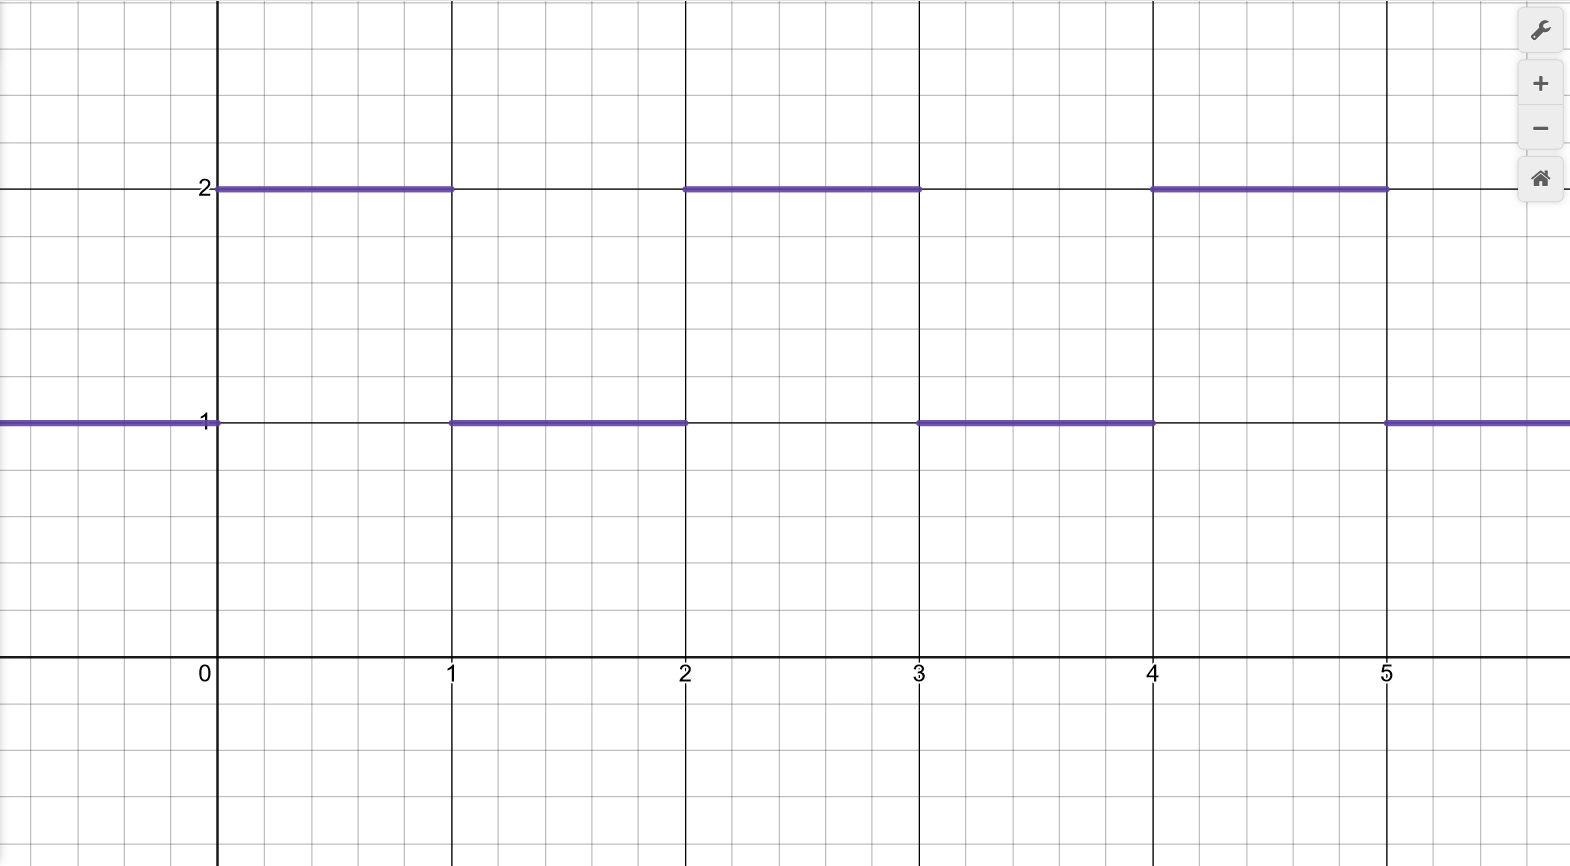
\includegraphics[width=0.9\linewidth]{pic/gr_1.png}}
\caption{График функции $f(t)$.}
\end{figure}

Рассмотрим частичные суммы Фурье $F_N$ и $G_N$ вида

\begin{equation}
F_N(t) = \frac{a_0}{2} + \sum  \limits_{n=1}^N \left( a_n \cos \left( \omega_n t \right) + b_n \sin \left( \omega_n t \right)  \right) \, ,
\end{equation}

\begin{equation}
G_N (t) = \sum  \limits_{n=-N}^N c_n e^{i \omega_n t} \, ,
\end{equation}
где $\omega_n = 2 \pi \frac{n}{T}$.\\
\\
Перепишем формулы выше с учетом того, что $T = 2 \pi$, следовательно  $\omega_n = 2 \pi \frac{n}{ 2 \pi} = n$:
\begin{equation}
F_N(t) = \frac{a_0}{2} + \sum  \limits_{n=1}^N \left( a_n \cos \left( n t \right) + b_n \sin \left( n t \right)  \right) \, ,
\end{equation}

\begin{equation}
G_N (t) = \sum  \limits_{n=-N}^N c_n e^{i n t}.
\end{equation}

Перейдем к разложению по формуле 4.\\
$f(x)$ определена на $[ \pi, 3\pi]$, преобразуем:
\begin{equation}
\pi \leq t \leq 3 \pi \to \pi - 2 \pi \leq t - 2 \pi \leq 3 \pi - 2 \pi \to -\pi \leq t - 2 \pi \leq \pi
\end{equation}
Новая переменная $x = t - 2\pi$. Выразим $t = x + 2 \pi$ и запишем новую функцию $\phi (x) = f (x + 2 \pi)$.
\begin{equation}
\phi (x) = \frac{a_0}{2} + \sum  \limits_{n=1}^N \left( a_n \cos \left( n x \right) + b_n \sin \left( n x \right)  \right) \, ,
\end{equation}
где $a_0, \, a_n, \, b_n$ -- коэффициенты Фурье:

\begin{equation}
a_0 = \frac{1}{\pi} \int \limits_{-\pi}^{\pi} \phi (x) dx,
\end{equation}
\begin{equation}
a_n = \frac{1}{\pi} \int \limits_{-\pi}^{\pi} \phi (x) \cos (n x) dx,
\end{equation}
\begin{equation}
b_n = \frac{1}{\pi} \int \limits_{-\pi}^{\pi} \phi (x) \sin (nx) dx,
\end{equation}

Проведем обратную замену $x = t - 2\pi$:

\begin{equation}
f(t) = \frac{a_0}{2} + \sum  \limits_{n=1}^N \left( a_n \cos \left( n ( t - 2\pi) \right) + b_n \sin \left( n ( t - 2\pi) \right)  \right)
\end{equation}
Воспользуемся периодичностью синуса и косинуса:
\begin{equation}
f(t) = \frac{a_0}{2} + \sum  \limits_{n=1}^N \left( a_n \cos \left( n t  \right) + b_n \sin \left( n  t  \right)  \right)
\end{equation}
\begin{equation}
a_0 = \frac{1}{\pi} \int \limits_{\pi}^{3\pi} f(t) dt,
\end{equation}
\begin{equation}
a_n = \frac{1}{\pi} \int \limits_{\pi}^{3\pi} f(t) \cos (n t) dt,
\end{equation}
\begin{equation}
b_n = \frac{1}{\pi} \int \limits_{\pi}^{3\pi} f(t) \sin (nt) dt,
\end{equation}
Вычислим значения коэффициентов:

\begin{equation}
a_0 = \frac{1}{\pi} \left( \int \limits_{\pi}^{2\pi} 1 dt + \int \limits_{2\pi}^{3\pi} 2 dt\right) =
 \frac{1}{\pi} \left( \pi + 2\pi \right) = 3,
\end{equation}

\begin{equation}
a_n = \frac{1}{\pi} \left( \int \limits_{\pi}^{2\pi} \cos (n t) dt +  2\int \limits_{2\pi}^{3\pi} \cos (n t) dt \right)
\end{equation}

Отдельно вычислим неопределенный интеграл:
\begin{equation}
\int \cos (n t) dt = \left| u = nt , t = \frac{u}{n},  dt = \frac{du}{n}\right| = \int  \frac{ \cos (u) du}{n} = \frac{\sin u}{n} + C = \frac{\sin (nt)}{n} + C
\end{equation}


Отсюда получим
\begin{equation}
a_n = \frac{1}{\pi} \left( \left. \frac{\sin (nt)}{n} \right|_{\pi}^{2\pi} +  2  \left. \frac{\sin (nt)}{n} \right|_{2\pi}^{3\pi} \right) = 0
\end{equation}



\begin{multline}
b_n = \frac{1}{\pi} \left( \int \limits_{\pi}^{2\pi} \sin (n t) dt +  2\int \limits_{2\pi}^{3\pi} \sin (n t) dt \right) =
-\frac{1}{\pi} \left( \left. \frac{\cos (nt)}{n} \right|_{\pi}^{2\pi} +  2  \left. \frac{\cos (nt)}{n} \right|_{2\pi}^{3\pi} \right) =\\
= -\frac{1}{\pi} \left( \frac{\cos (2 \pi n) - \cos (\pi n)}{n} +  2 \frac{\cos (3 \pi n) - \cos (2 \pi n)}{n} \right) = \\
= -\frac{1}{\pi} \left( \frac{ 1 - \cos (\pi n)}{n} +  2 \frac{\cos (3 \pi n) - 1}{n} \right) =
-\frac{1}{\pi} \left( \frac{ 1 - (-1)^n}{n} +  2 \frac{(-1)^n - 1}{n} \right) =\\
= -\frac{1}{\pi} \left( \frac{(-1)^n - 1 }{n} \right) = \frac{1 - (-1)^n}{\pi n}
\end{multline}
Примеры вычисления первых значений $b_n$:
\begin{equation}
b_1 = \frac{1 - (-1)^1}{\pi} = \frac{2}{\pi}
\end{equation}
\begin{equation}
b_2 = \frac{1 - (-1)^2}{2\pi} = 0
\end{equation}
\begin{equation}
b_3 = \frac{1 - (-1)^3}{3\pi} = \frac{2}{3\pi}
\end{equation}
\begin{equation}
b_0 = \frac{1}{\pi} \left( \int \limits_{\pi}^{2\pi} \sin (0) dt +  2\int \limits_{2\pi}^{3\pi} \sin (0) dt \right)  = 0
\end{equation}

Запишем получившуюся частичную сумму:
\begin{equation}
F_N(t) = \frac{3}{2} + \sum  \limits_{n=1}^N \left( \frac{1 - (-1)^n}{\pi n} \sin \left( n t \right)  \right) \, ,
\end{equation}
\\
Перейдем к рассмотрению следующей частичной суммы:
\begin{equation}
G_N (t) = \sum  \limits_{n=-N}^N c_n e^{i n t}.
\end{equation}
Где соответствующий коэффициент:
\begin{equation}
c_n = \frac{1}{T} \int \limits_{h}^{h + T} f(t) e^{i \omega_n t} dt = \frac{1}{2 \pi} \int \limits_{\pi}^{3 \pi} f(t) e^{i n t} dt =
\frac{1}{2 \pi} \left( \int \limits_{\pi}^{2 \pi} e^{i n t} dt + 2 \int \limits_{ 2 \pi}^{3 \pi} e^{i n t} dt \right) 
\end{equation}

Отдельно вычислим неопределенный интеграл:
\begin{equation}
c_n = \int e^{i n t} dt = \frac{1}{in} \int e^{i n t} d (i n t) =  \frac{e^{i n t}}{in} + C
\end{equation}

\begin{equation}
c_n = \frac{1}{2 \pi} \left(  \left. \frac{e^{i n t}}{in} \right|_{\pi}^{2\pi} + 2  \left. \frac{e^{i n t}}{in} \right|_{2\pi}^{3\pi} \right) =
 \frac{ 2 e^{3i n \pi} - e^{i n \pi} - e^{2i n \pi}}{2 i n \pi}
\end{equation}

В итоге полученое разложение:
\begin{equation}
G_N (t) = \sum  \limits_{n=-N}^N  \frac{ 2 e^{3i n \pi} - e^{i n  \pi} - e^{2i n \pi}}{2 i n \pi} e^{i n t}.
\end{equation}






\newpage
\subsection{Любая четная периодическая функция.}
\begin{equation}
f(t) = \cos t
\end{equation}

\begin{figure}[h]
\center{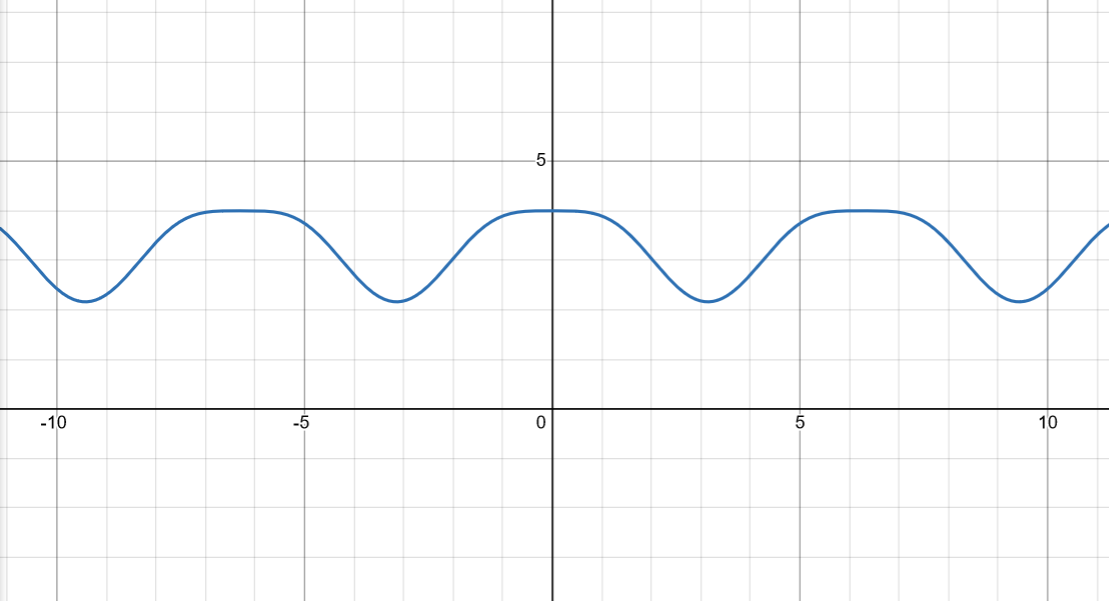
\includegraphics[width=0.9\linewidth]{pic/gr_2.png}}
\caption{График функции $f(t)$.}
\end{figure}





\newpage
\subsection{Любая нечетная периодическая функция.}
\begin{equation}
f(t) = \sin t
\end{equation}

\begin{figure}[h]
\center{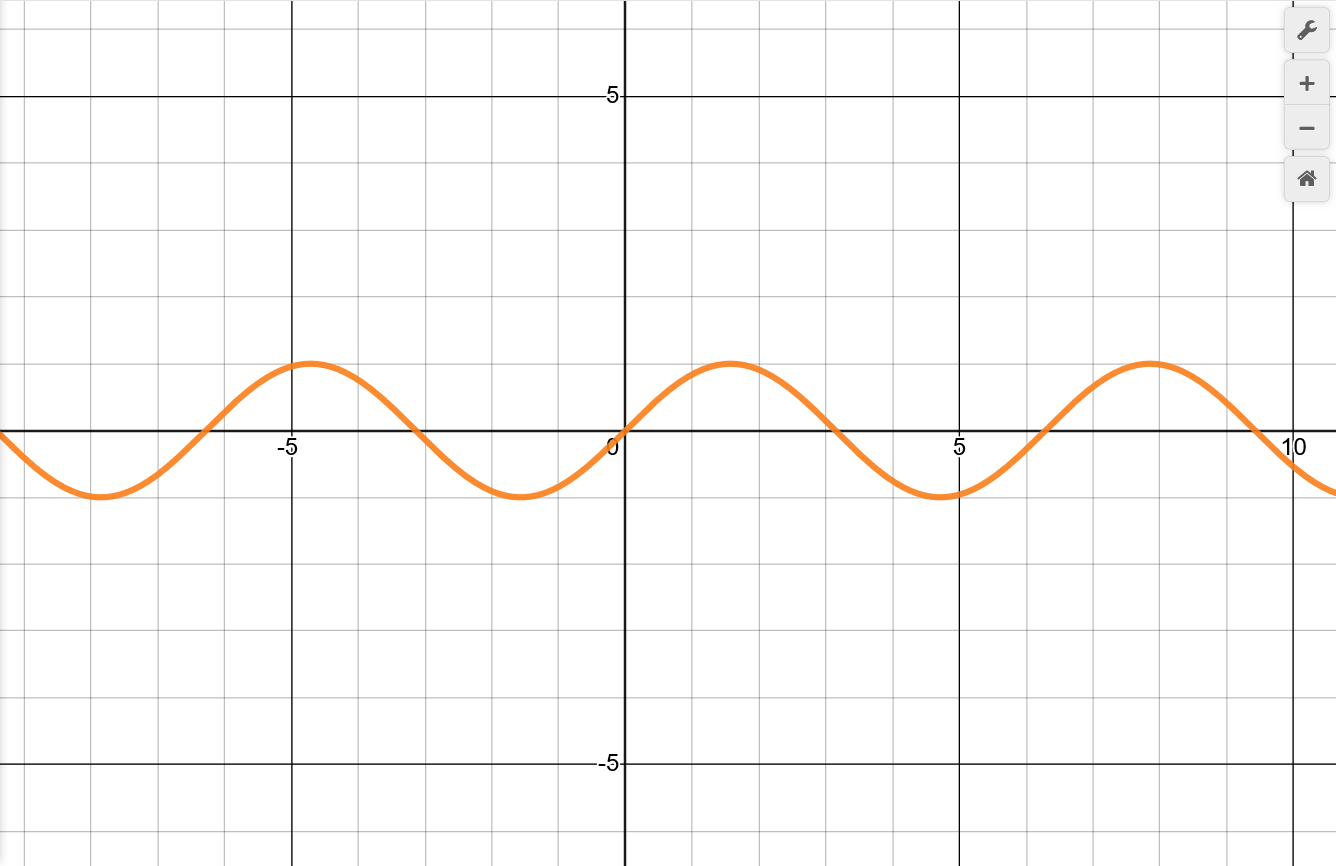
\includegraphics[width=0.9\linewidth]{pic/gr_3.png}}
\caption{График функции $f(t)$.}
\end{figure}





\newpage
\subsection{Любая периодическая функция, график которой состоит не только из прямых линий, и которая не является ни четной, ни нечетной.}
\begin{equation}
f(t) = \cos (t + 1)
\end{equation}

\begin{figure}[h]
\center{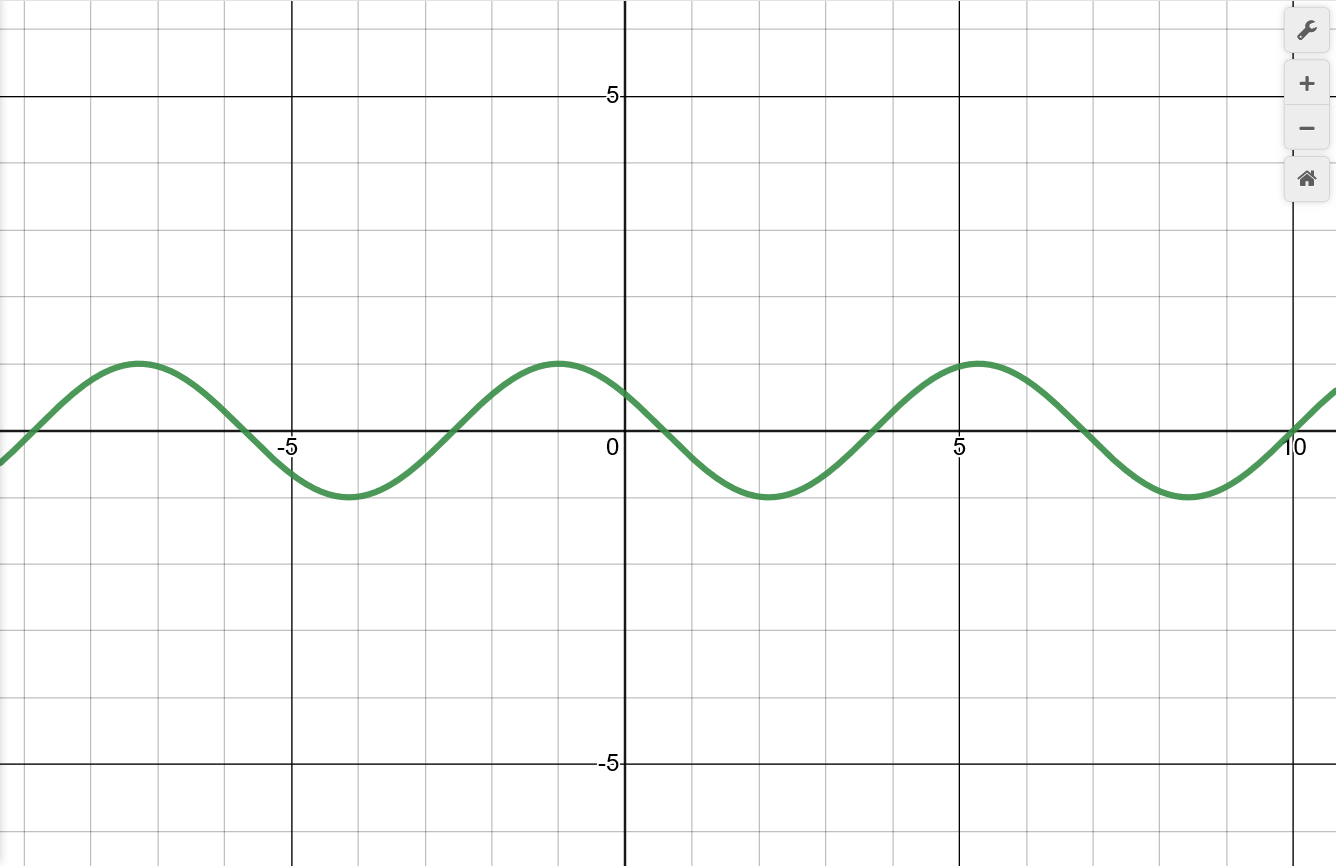
\includegraphics[width=0.9\linewidth]{pic/gr_4.png}}
\caption{График функции $f(t)$.}
\end{figure}


%\begin{center}
%\begin{lstlisting}[label=some-code,caption={Исходный код для 1207}]
%\end{lstlisting}
%\end{center}

%\begin{figure}[h]
%\center{\includegraphics[width=0.9\linewidth]{pic/screen_1296.png}}
%\caption{Результат отправки задачи 1296.}
%\end{figure}

 
\end{document}













